% XCircuit output "config6xy.tex" for LaTeX input from config6xy.ps
\def\putbox#1#2#3#4{\makebox[0in][l]{\makebox[#1][l]{}\raisebox{\baselineskip}[0in][0in]{\raisebox{#2}[0in][0in]{\scalebox{#3}{#4}}}}}
\def\rightbox#1{\makebox[0in][r]{#1}}
\def\centbox#1{\makebox[0in]{#1}}
\def\topbox#1{\raisebox{-0.60\baselineskip}[0in][0in]{#1}}
\def\midbox#1{\raisebox{-0.20\baselineskip}[0in][0in]{#1}}
   \scalebox{1}{
   \normalsize
   \parbox{4.1875in}{
   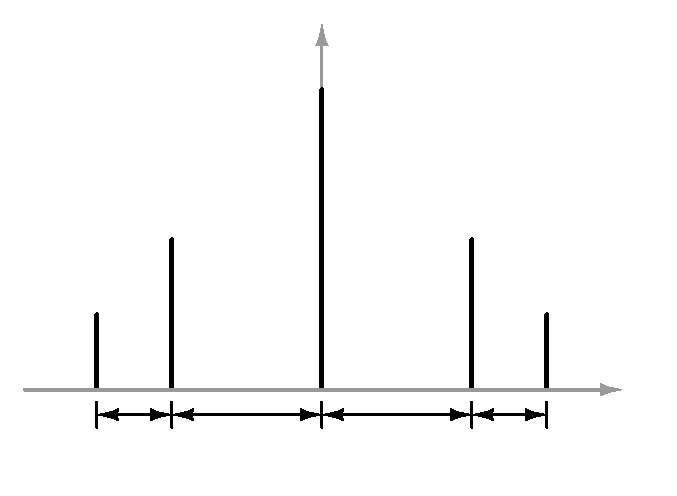
\includegraphics[scale=1]{config6xy}\\
   % translate x=540 y=424 scale 0.38
   \putbox{1.85in}{0.7in}{1.20}{\rotatebox{-270}{\tiny{$\lambda = \SI{3.75}{\meter}$}}}%
   \putbox{0.85in}{0.7in}{1.20}{\rotatebox{-270}{\tiny{$\lambda /2 = \SI{1.875}{\meter}$}}}%
   \putbox{0.35in}{0.7in}{1.20}{\rotatebox{-270}{\tiny{$\lambda /4 = \SI{0.9375}{\meter}$}}}%
   \putbox{2.85in}{0.7in}{1.20}{\rotatebox{-270}{\tiny{$\lambda /2 = \SI{1.875}{\meter}$}}}%
   \putbox{3.4in}{0.7in}{1.20}{\rotatebox{-270}{\tiny{$\lambda /4 = \SI{0.9375}{\meter}$}}}%
   \putbox{2.14in}{2.89in}{1.20}{$z$}%
   \putbox{4.14in}{0.56in}{1.20}{$x$}%
   \putbox{1.2in}{0.26in}{1.20}{{\tiny{$\lambda /2 = \SI{1.875}{\meter}$}}}%
   \putbox{2.2in}{0.26in}{1.20}{{\tiny{$\lambda /2 = \SI{1.875}{\meter}$}}}%
   \putbox{0.58in}{0.26in}{1.20}{\tiny{$\lambda /4=$}}%
   \putbox{3.18in}{0.26in}{1.20}{\tiny{$\lambda /4=$}}%
   \putbox{0.5in}{0.15in}{1.20}{\tiny{$\SI{0.9375}{\meter}$}}%
   \putbox{3.1in}{0.15in}{1.20}{\tiny{$\SI{0.9375}{\meter}$}}%
   } % close 'parbox'
   } % close 'scalebox'
   \vspace{-\baselineskip} % this is not necessary, but looks better
